%!TEX root = ../../diss.tex

\chapter[The End - A Sermon]{The End - A Sermon}\label{chap:the_end}


Lorem Epson. 

\begin{figure}[htpb]
	\centering
	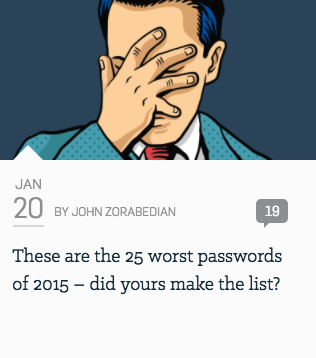
\includegraphics[width=0.3\linewidth]{shaming/nakedsecurity-sophos}
	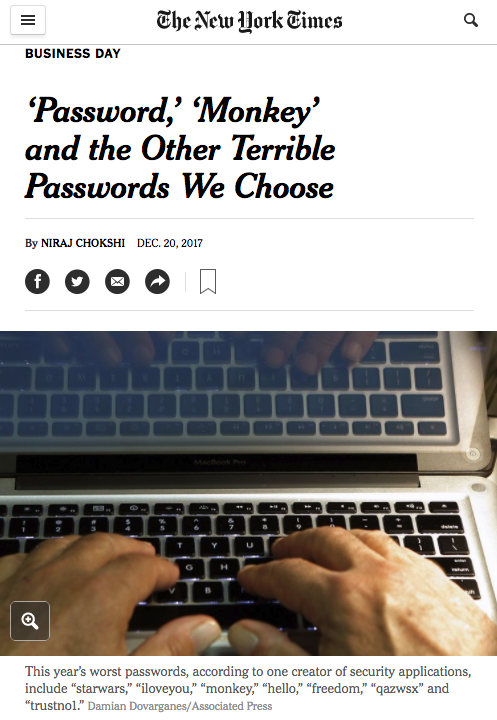
\includegraphics[width=0.3\linewidth]{shaming/nytimes}
	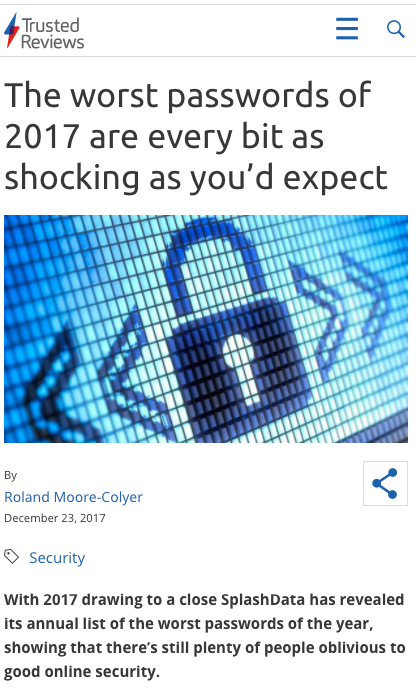
\includegraphics[width=0.3\linewidth]{shaming/trusted-reviews}
\end{figure}

Key thoughts

\begin{itemize}
\item Passwords are bad. Let's hope passwords vanish at some point. Make machines intelligent enough to decide if a user should be granted access or not. But this brings new problems.
\item Maybe passwords are the vinyl records of usable security - everyone agrees that it's kind of an obsolete technology but there's something to it that ensure they don't disappear. %TODO come up with a better analogy.
 \item  if passwords become obsolete tomorrow, many of us will not grief. 
 \item  the media should stop shaming the users 
 \item  it's okay to forget passwords! reference to the article Franziska shared with me (SZ,  01.12.2017 ``Die Kunst zu vergessen'' \footurl{http://www.sueddeutsche.de/wissen/neurowissenschaft-die-kunst-zu-vergessen-1.3772438}{02.01.2018}.)
 \item 	ad networks for webpages can undermine any attempt to secure one's account. Too many websites show ads that can run harmful scripts. yes, adblockers do prevent this, but not everyone has one installed (especially novice users don't). Frightening research on this: \footurl{https://freedom-to-tinker.com/2017/12/27/no-boundaries-for-user-identities-web-trackers-exploit-browser-login-managers/}{02.01.2018}
\end{itemize}


%TODO I have more thann 100 ``takeaways'' from papers. This could be a funny ``sermon'' too (Luther's 100 theses);


